\documentclass[submit]{harvardml}

\course{CS181-S24}
\assignment{Assignment \#5}
\duedate{11:59pm EST, April 12, 2024}
\newcommand{\attr}[1]{\textsf{#1}}
\usepackage[OT1]{fontenc}
\usepackage[colorlinks,citecolor=blue,urlcolor=blue]{hyperref}
\usepackage[pdftex]{graphicx}
\usepackage{subfig}
\usepackage{framed}
\usepackage{fullpage}
\usepackage{amsmath}
\usepackage{amssymb}
\usepackage{color}
\usepackage{todonotes}
\usepackage{listings}
\usepackage{common}
\usepackage{bm}
\usepackage{tikz}
\usetikzlibrary{bayesnet}
\usepackage{pythonhighlight}
\usetikzlibrary{positioning,shapes,arrows}

\usepackage[mmddyyyy,hhmmss]{datetime}

\definecolor{verbgray}{gray}{0.9}

\lstnewenvironment{csv}{%
  \lstset{backgroundcolor=\color{verbgray},
  frame=single,
  framerule=0pt,
  basicstyle=\ttfamily,
  columns=fullflexible}}{}

\begin{document}
\begin{center}
{\Large Homework 5: Mixtures, EM, and Graphical Models}\\
\end{center}

\subsection*{Introduction}

This homework assignment will have you work with EM for mixtures, PCA,
and graphical models.

\subsection*{Resources and Submission Instructions}

We encourage you to read sections 9.4 and 8.2.5 of the course textbook.

Please type your solutions after the corresponding problems using this
\LaTeX\ template, and start each problem on a new page.

Please submit the \textbf{writeup PDF to the Gradescope assignment `HW5'}. Remember to assign pages for each question.

Please submit your \textbf{\LaTeX\ file and code files to the Gradescope assignment `HW5 - Supplemental'}. 


\begin{problem}[Expectation-Maximization for Gamma Mixture Models: Derivations, 10pts]

In this problem we will explore expectation-maximization for a Categorical-Gamma Mixture model.

Let us suppose the following generative story for an observation $x$: first one of $K$ classes is randomly selected, and then the features $x$ are sampled according to this class. If $$z \sim \operatorname{Categorical}(\btheta)$$ indicates the selected class, then $x$ is sampled according to the class or ``component'' distribution corresponding to $z$. (Here, $\btheta$ is the mixing proportion over the $K$ components: $\sum_k \theta_k = 1$ and $ \theta_k > 0$). In this problem, we assume these component distributions are gamma distributions with shared shape parameter but different rate parameters: $$x | z \sim \operatorname{Gamma}(\alpha, \beta_k).$$

In an unsupervised setting, we are only given a set of observables as our training dataset: $\mathcal D = \{x_n\}_{n=1}^N$. The EM algorithm allows us to learn the underlying generative process (the parameters $\btheta$ and $\{\beta_k\}$) despite not having the latent variables $\{z_n\}$ corresponding to our training data.

\vspace{2em}

\begin{enumerate}

  \item \textbf{Intractability of the Data Likelihood} We are
    generally interested in finding a set of parameters $\beta_k$ that
    maximizes the likelihood of the observed data: $$\log
    p(\{x_n\}^N_{n=1}; \btheta, \{\beta_k\}^K_{k = 1}).$$ Expand the data
    likelihood to include the necessary sums over observations
    $x_n$ and to marginalize out the latents
    $\boldz_n$. Why is optimizing this likelihood directly
    intractable?

\item \textbf{Complete Data Log Likelihood} The complete dataset
  $\mathcal D = \{(x_n, \boldz_n)\}_{n=1}^N$ includes latents $\boldz_n$. Write
  out the negative complete data log likelihood: $$\mcL(\btheta, \{\beta_k\}^K_{k=1}) =  -\log p(\mathcal D; \btheta, \{\beta_k\}^K_{k=1}).$$

  Apply the power trick and simplify your expression using indicator elements $z_{n
  k}$.\footnote{The ``power trick'' is used when terms in a PDF are raised to the power of indicator components of a one-hot vector.  For example, it allows us to rewrite $p(\boldz_n ;  \btheta) = \prod_k \theta_k^{z_{nk}}$.} Notice that optimizing this loss is now computationally tractable if we know $\boldz_n$.

  (Continued on next page.)

\end{enumerate}

\end{problem}

\newpage


\begin{framed}
\noindent\textbf{Problem 1} (cont.)\\
\begin{enumerate}
\item[3.] \textbf{Expectation Step} Our next step is to introduce a
  mathematical expression for $\boldq_n$, the posterior over the
  hidden component variables~$\boldz_n$ conditioned on the observed data
  $x_n$ with fixed parameters.
That is:
  \begin{align*}
    \textbf{q}_n &= \begin{bmatrix}
      p(\boldz_n =\boldC_1| x_n; \btheta, \{ \beta_k \}^K_{k=1}) \\
      \vdots \\
      p(\boldz_n =\boldC_K| x_n; \btheta, \{ \beta_k \}^K_{k=1})
    \end{bmatrix}.
  \end{align*}
  %
%
  Write down and simplify the expression for
  $\boldq_n$.  Note that because the $\boldq_n$ represents the
  posterior over the hidden categorical variables $\boldz_n$, the
  components of vector $\boldq_n$ must sum to 1.
  The main work is to find an expression for $p(\boldz_n|x_n; \btheta, \{\beta_k\}^K_{k=1})$  for any choice of $\boldz_n$; i.e., for any 1-hot encoded $\boldz_n$. With this, you can then construct the different components that make up the vector $\boldq_n$.
  
\item[4.] \textbf{Maximization Step}
Using the~$\boldq_n$ estimates from the Expectation Step, derive an update for maximizing the expected complete data log likelihood in terms of $\btheta$ and $\{ \beta_k \}^K_{k=1}$.

\begin{enumerate}
    \item Derive an expression for the expected complete data log likelihood using $\boldq_n$.
    \item Find an expression for $\btheta$ that maximizes this expected complete data log likelihood. You may find it helpful to use Lagrange multipliers in order to enforce the constraint $\sum \theta_k = 1$. Why does this optimal $\btheta$ make intuitive sense?
    \item Find an expression for $\beta_k$ that maximizes the expected complete data log likelihood.  Why does this optimal $\beta_k$  make intuitive sense?
\end{enumerate}
    
\item[5.] Suppose that this had been a classification problem. That is,
  you were provided the ``true'' components $\boldz_n$ for each
  observation $x_n$,
  and you were going to perform the classification by
  inverting the provided generative model (i.e. now you're predicting $\boldz_n$ given $x_n$). Could you reuse any of
  your derivations above to estimate the parameters of the model?
  
\end{enumerate}
  
\end{framed}

\newpage 
\textbf{Q1}
\subsection*{Solution}

\begin{enumerate}
  \item Given the data likelihood for a set of observations $\{x_i\}_{i=1}^N$ and parameters $\theta$ and $\{\beta_k\}_{k=1}^K$:

\begin{equation}
    \log p(\{x_i\}_{i=1}^N; \theta, \{\beta_k\}_{k=1}^K).
\end{equation}

We introduce latent variables $\{z_i\}_{i=1}^N$ that require marginalization:

\begin{equation}
    p(\{x_i\}_{i=1}^N; \theta, \{\beta_k\}_{k=1}^K) = \sum_{i=1}^N \log \left( \sum_{k=1}^K p(x_i | z_i=k; \theta) p(z_i=k; \beta_k) \right).
\end{equation}

Direct optimization of this likelihood is not tractable because the latent variable $z_i$ is nested inside the logarithm. Differentiating through the logarithm of the sum is mathematically challenging especially in programs, making separation of terms for optimization difficult, as indicated in equation (9.3.1) (class). 
  \item Consider a dataset \( \mathcal{D} = \{(x_i, z_i)\}_{i=1}^M \) with associated latent variables \( z_i \). The negative log likelihood of the complete data with parameters \( \phi \) and \( \{\alpha_l\}_{l=1}^L \) is given by:

\begin{equation}
    \mathcal{L}(\phi, \{\alpha_l\}_{l=1}^L) = -\log p(\mathcal{D}; \phi, \{\alpha_l\}_{l=1}^L).
\end{equation}

Applying the 'power trick' and using the indicator variable \( z_i^l \), decompose the likelihood as follows:

\begin{equation}
    \mathcal{L}(\phi, \{\alpha_l\}_{l=1}^L) = -\sum_{i=1}^M \log \left( \prod_{l=1}^L [p(x_i | z_i=l; \phi) p(z_i=l; \alpha_l)]^{z_i^l} \right).
\end{equation}

This results in a tractable optimization problem for the negative log likelihood when \( z_i \) is known:

\begin{equation}
    \mathcal{L}(\phi, \{\alpha_l\}_{l=1}^L) = -\sum_{i=1}^M \left( \sum_{l=1}^L z_i^l \log \Gamma(x_i; \alpha_l, \phi_l) \right).
\end{equation}

Through doing so, I have seperated the terms and can now continue optimization. 
  \item Given a dataset with observations $\{y_i\}_{i=1}^M$ and fixed parameters $\phi$ and $\{\gamma_j\}_{j=1}^J$, I will express the posterior distribution $r_i$ over the hidden variables $w_i$ conditioned on $y_i$. That is,

\begin{equation}
r_i = 
\begin{bmatrix}
\frac{p(w_i = H_1 | y_i; \phi, \{\gamma_j\}_{j=1}^J)}{\sum_{j=1}^J p(w_i = H_j | y_i; \phi, \{\gamma_j\}_{j=1}^J)} \\
\vdots \\
\frac{p(w_i = H_J | y_i; \phi, \{\gamma_j\}_{j=1}^J)}{\sum_{j=1}^J p(w_i = H_j | y_i; \phi, \{\gamma_j\}_{j=1}^J)}
\end{bmatrix}.
\end{equation}

To calculate $r_i$, first determine the conditional probability for each hidden variable state $H_j$; for any one-hot encoded $w_i$, apply Bayes' theorem:

\begin{equation}
p(w_i | y_i; \phi, \{\gamma_j\}_{j=1}^J) = \frac{p(y_i | w_i = H_j; \phi) p(w_i = H_j; \gamma_j)}{\sum_{j=1}^J p(y_i | w_i = H_j; \phi) p(w_i = H_j; \gamma_j)}.
\end{equation}

The components of the posterior vector $r_i$ sum to one, as they represent the probability distribution over the hidden categorical variables $w_i$.
  \item \begin{enumerate}
      \item Given the estimates from the Expectation Step, I will maximize the expected complete data log likelihood for the parameters \( \psi \) and \( \{\lambda_l\}_{l=1}^L \).

Define the expected complete data log likelihood as:
\begin{equation}
    Q(\psi, \{\lambda_l\}_{l=1}^L) = \mathbb{E}_{Y|X, \psi, \{\lambda_l\}_{l=1}^L}[\log p(X, Y; \psi, \{\lambda_l\}_{l=1}^L)].
\end{equation}

This expectation can be rewritten using the posterior probabilities \( r_{il} \) computed in the Expectation Step:
\begin{equation}
    Q(\psi, \{\lambda_l\}_{l=1}^L) = \sum_{i=1}^M \sum_{l=1}^L r_{il} \log p(x_i | y_i = H_l; \psi) p(y_i = H_l; \lambda_l),
\end{equation}
where \( r_{il} = p(y_i = H_l | x_i; \psi, \{\lambda_l\}_{l=1}^L) \) is the posterior probability that the latent variable \( y_i \) is in state \( H_l \).

This maximization step leads to updated parameter estimates for \( \psi \) and \( \{\lambda_l\}_{l=1}^L \) by optimizing the expected log likelihood.
      \item To optimize the parameters \( \phi \) for our model, I will maximize the expected complete data log likelihood, which includes a constraint that the sum of \( \phi \) over all categories must be 1.

The optimization is performed by setting the derivative of the Lagrangian to zero:

\begin{equation}
    \frac{\partial}{\partial \phi_k} \left[ \sum_{i=1}^M \sum_{j=1}^J r_{i,j} \log(\text{Gamma}(y_i; \alpha_j, \phi_j)) + \log(\phi_j) \right] + \nu \left( \sum_{j=1}^J \phi_j - 1 \right) = 0
\end{equation}

Solving for \( \phi_k \):

\begin{equation}
    -\frac{1}{\nu} \sum_{i=1}^M r_{i,k} = \phi_k
\end{equation}

Using the fact that the sum of all \( \phi_k \) is constrained to 1:

\begin{equation}
    1 = \sum_{j=1}^J \phi_j = -\frac{1}{\nu} \sum_{j=1}^J \sum_{i=1}^M r_{i,j}
\end{equation}

Therefore:

\begin{equation}
    \nu = -M
\end{equation}

And thus, the optimal \( \phi_k \) is given by:

\begin{equation}
    \phi_k = \frac{1}{M} \sum_{i=1}^M r_{i,k}
\end{equation}

This solution makes intuitive sense as it reflects the average probability of a data point belonging to class \( k \) across all observations.
      \item Given the expected complete data log likelihood, find the parameter \( \mu_k \) that maximizes this function under the constraint that the sum of all \( \mu_k \) equals 1. Apply the derivative with respect to \( \mu_k \) and introduce a Lagrange multiplier \( \nu \) to enforce the constraint.

\begin{equation}
    \frac{\partial}{\partial \mu_k} Q(\varphi, \{\mu_l\}_{l=1}^L) = \frac{\partial}{\partial \mu_k} \left[ \sum_{i=1}^M \sum_{l=1}^L s_{i,l} \log(\text{Gamma}(y_i; \alpha, \mu_l)) + \nu \left( \sum_{l=1}^L \mu_l - 1 \right) \right] = 0
\end{equation}

Solving for \( \mu_k \):

\begin{equation}
    \frac{1}{\mu_k} \sum_{i=1}^M s_{i,k} \alpha = \sum_{i=1}^M s_{i,k} y_i
\end{equation}

Rearranging for the optimal \( \mu_k \):

\begin{equation}
    \mu_k = \frac{\sum_{i=1}^M s_{i,k} y_i}{\sum_{i=1}^M s_{i,k} \alpha}
\end{equation}

This expression aligns with the intuitive understanding that \( \mu_k \) should reflect the average behavior of data points assigned to the k-th component.

  \end{enumerate}
  \item In a classification scenario with known labels \( w_i \) corresponding to each observation \( y_i \), we can circumvent the iterative nature of the EM algorithm. Given \( w_i \), parameter estimation simplifies by directly applying the maximization step, utilizing the relations derived for expected log likelihood. This eliminates the need for alternating between expectation and maximization steps, enabling a direct computation of model parameters.

\end{enumerate}


\newpage

\begin{problem}[Expectation-Maximization for Gamma Mixture Models: Coding, 15 pts]

  In this problem, you will implement your EM derivations from Problem
  1 and apply it to analyzing a synthetic example of the recovery time
  for patients following a surgical procedure, in hours.  The doctors
  have noticed that some patients seem to recover at an expected rate,
  but sometimes the recovery takes a long time.  They are keen to
  understand what is going on to improve their processes.  
  
  \begin{enumerate}

  \item Plot the data.  How would you describe the distribution?
    Based on what you see, why might a mixture model be an appropriate
    model?  
    
  \item Implement your solution from Problem 1 in \texttt{homework5.ipynb}.

{\bfseries You will recieve no points for code not included below.}

 
\item Run your code for 1, 2, 3, and 4 mixture components.  Plot the
  mixture models you find on top of the data distribution as well as
  the associated log likelihoods.  How many mixtures does it seem that
  there are?  How would you decide?
  
\item The doctors tell you that a normal recovery from the procedure
  is about 2-3 days, though sometimes patients recover a little
  faster.  Does this match what you see in the data?  Provide some
  hypotheses about what might be going on.

\item It's clear from the data that some patients take significantly
  longer than 2-3 days.  Do you observe that there is evidence that
  these represent a different cluster, vs. a long tail from a single
  cluster?  Why or why not?

\item The physician-scientists want to use this model to understand
  the characteristics of patients who have very long recoveries
  vs. those who do not.  Is this mixture modeling approach appropriate
  for this task?  Why or why not?

\item The physician-scientists develop a way of identifying someone's
  cluster based on a blood test---it seems that some patients in the
  longer group are ones that are at risk for clotting-related
  complications.  The hospital operations staff want to use this model
  to help streamline operations.  They plan to use the cluster of the
  patient to predict which patients will have a long length of stay.
  Is this plan sound?  May there be some issues?
  
  \end{enumerate} 
  
\end{problem} 

\newpage
\textbf{Q2}
\subsection*{Solution}

\begin{enumerate}
  \item The histogram of recovery times is a skewed distribution that's concentrated at lower values with a long right tail. This pattern suggests the presence of at least two subpopulations: one recovering quickly and another taking much longer. A mixture model, therefore, is well-suited to model this data, as it can accommodate multiple underlying distributions, each corresponding to different recovery profiles.
 Plot: \includegraphics[width=0.5\linewidth]{hw5/1.png}
  
  \item 
Code:

    \begin{python}
def e_step(theta, betas):
    q = ds.Gamma(alpha, betas).log_prob(x) + theta.log() 
    q = q - q.logsumexp(dim=1, keepdim=True)
    q = q.exp() 
    return q


def m_step(q):
    theta_hat = q.mean(dim=0)
    betas_hat = (alpha * q.sum(dim=0)) / (q * x.unsqueeze(-1)).sum(dim=0)
    return theta_hat, betas_hat

def log_px(x, theta, betas):
    p = torch.zeros(x.shape[0], len(betas))
    for k in range(len(betas)):
        gamma_dist = ds.Gamma(alpha, betas[k])
        p[:, k] = theta[k] * gamma_dist.log_prob(x).exp()
    return torch.log(p.sum(dim=1))


def run_em(theta, betas, iterations=1000):
   for _ in range(iterations):
        q = e_step(theta, betas)
        theta, betas = m_step(q)
    return theta, betas
    \end{python}
  \item Plots: \includegraphics[width=0.5\linewidth]{hw5/2.png} \includegraphics[width=0.5\linewidth]{hw5/3.png} \includegraphics[width=0.5\linewidth]{hw5/4.png} \includegraphics[width=0.5\linewidth]{hw5/5.png}
  The overlay plots suggest that the model with three mixture components fits the data well without overfitting, as shown by a better capture of the distribution's shape compared to one or two components and no significant improvement with four components. The choice of the number of mixtures is best guided by a balance between model complexity and goodness of fit, usually by AIC or BIC.
  \item The recovery time data indicates a pronounced peak around 40-50 hours, suggesting a common recovery period that aligns with the expected 2-3 day timeframe. An additional, less plausible peak near zero hours prompts speculation of data entry errors or procedural cancellations, which shows the need for data cleansing measures such as filtering out these arbitrarily low values before analysis.
  \item The data does indicate a subgroup experiencing extended recovery times, which is distinct from the primary cluster recovering within 2-3 days. With $K=3$, the parameter estimation allocates non-negligible probability to a third cluster, as reflected by the estimated mixture proportions and distinct parameter values for the third component. The presence of this third cluster, rather than a single elongated tail of the distribution, is thus influenced by the discrete nature of the additional peak in the histogram.
  \item Yes, mixture modeling is apt for distinguishing between patient recovery profiles. This is because it employs a hidden variable, represented as \( z \), which probabilistically classifies recovery times into distinct groups. The model's ability to assign recovery times to different components based on \( \theta \) values like 16\%, 74\%, and 10\% suggests it can differentiate between varying recovery durations. Such probabilistic assignments enable the identification of patient characteristics associated with each group, offering insights into the factors affecting recovery length.
  \item While the physicians' blood test identification for patient clusters could enhance the understanding of recovery risks, the operational use of this model may encounter obstacles. Variability within the long recovery cluster and the overlap with shorter recovery clusters could challenge how accurate length-of-stay predictions actually end up being. Also, uniform distribution across a wide range of the long recovery times might diminish the model's precision in operational planning.

\end{enumerate}


\newpage
  
\begin{problem}[PCA, 15 pts]

  
For this problem you will implement PCA from scratch on the first 6000 images of the MNIST dataset. Your job is to apply PCA on MNIST and discuss what kind of structure is found. Implement your solution in \texttt{homework5.ipynb} and attach the final plots below.

{\bfseries You will recieve no points for using third-party PCA implementations (i.e. {\normalfont \texttt{scikit-learn}}).}

{\bfseries You will receive no points for code not included below.}
\begin{enumerate}

\item Compute the PCA. Plot the eigenvalues corresponding to the most
  significant 500 components in order from most significant to
  least. Make another plot that describes the cumulative proportion of
  variance explained by the first $k$ most significant components for
  values of $k$ from 1 through 500.  How much variance is explained by
  the first 500 components?  Describe how the cumulative proportion of
  variance explained changes with $k$.  Include this plot below.

\item Plot the mean image of the dataset and plot an image
  corresponding to each of the first 10 principle components.  How do
  the principle component images compare to the cluster centers from
  K-means? Discuss any similarities and differences.  Include these
  two plots below.
  
  \textit{Reminder: Center the data before performing PCA}

\item Compute the reconstruction error on the data set using the mean
  image of the dataset.  Then compute the reconstruction error using
  the first 10 principal components.  How do these errors compare to
  the final objective loss achieved by using K-means on the dataset?
  Discuss any similarities and differences.

  For consistency in grading, define the reconstruction error as the squared L2
  norm averaged over all data points.


\item Suppose you took the original matrix of principle components
  that you found $U$ and multiplied it by some rotation matrix $R$.
  Would that change the quality of the reconstruction error in the
  last problem?  The interpretation of the components?  Why or why
  not?

\item Let's recall the zipcode application in Homework 3.  A common
  application of PCA is to dimensionality reduction before running a
  classifier: You first project the data onto the first few PCA bases,
  and then you train a classifier from the projection to the output.
  How might this be better than associating digits to clusters, as you
  did in Homework 4?  Would this approach help with any of the attacks
  in Homework 3?

\item You are collaborating with a penmanship analysis expert.  They
  are able to identify the kind of pen used to make a mark by various
  characteristics such as the width of the line, its crispness, and
  the type (if any) of ink splatter.  They have heard that your
  machine learning helped automate reading zip codes for the post
  office; they are wondering if you can help automate the manual
  process of classifying pen types.
  \begin{enumerate}
    \item Does what the expert is describing correspond to some kind
      of hidden representation or latent variable?  Describe why or
      why not.
    \item Do you think PCA will help the expert?  Why or why not?
      
  \end{enumerate}
\end{enumerate}
\end{problem}

\subsection*{Solution}
Code:

\begin{python}
def pca(x, n_comps=500):
    top_eigvals = 'not implemented'
    top_pcomps = 'not implemented'
    return top_eigvals, top_pcomps


def calc_cfvs(eigvals):
    cum_frac_vars = 'not implemented'
    return cum_frac_vars


def calc_errs(x, pcomps):
    err_mean = 'not implemented'
    err_pcomp = 'not implemented'
    return err_mean, err_pcomp
\end{python}

\begin{enumerate}
  \item Plots: \includegraphics[width=0.5\linewidth]{hw5/6.png} The plots reveal that the principal components up to the 500th account for nearly all the variance in the dataset, indicating a steep initial decline in the eigenvalues. The cumulative variance plot approaches a value close to 1, suggesting that these components capture the essence of the data. As $k$ increases, the growth rate of the explained variance diminishes, showing that each additional component contributes less to the total variance, which is expected in principal component analysis.
  \item Plots: \includegraphics[width=0.5\linewidth]{hw5/7.png} The principal components extracted from PCA do not resemble individual digits but rather capture the axes of maximum variance in the dataset. Unlike the distinct digit images formed by K-means cluster centers, these PCA components represent abstract features such as edges or curves common across numbers. This discrepancy illustrates the difference between identifying discrete clusters in the data (K-means) and finding orthogonal directions that maximize data variance (PCA).

  \item Reconstruction error (using mean): 4.382684e+06
        Reconstruction error (using mean and top 10 pcomps): 2.649772e+06
        The reconstruction errors indicate PCA's ability to better encapsulate the dataset's variance compared to the mean image. Using only the mean yields a high reconstruction error of approximately \(4.38 \times 10^6\), showing a large loss of information. Incorporating the first 10 principal components reduces this error to about \(2.65 \times 10^6\), which shows PCA’s aptness for data representation. When juxtaposed with K-means, which from previous computations showed a reduction in error from \(3.45 \times 10^6\) to \(2.60 \times 10^6\) with more iterations, PCA proves to be more effective, likely because of its mechanism of capturing maximum data variance via orthogonal transformations. Despite the computational demands of PCA, the lower reconstruction errors emphasize its efficiency and make it more suitable for feature extraction and dimensionality reduction than K-means clustering.
  \item Applying a rotation matrix \( R \) to the principal component matrix \( U \) does not alter the reconstruction error because the rotation maintains the vector norms, and thereby, the variance encapsulated by the components is unchanged. Mathematically, as rotation matrices are orthogonal, \( R^TR = RR^T = I \), which preserves the dot product, indicating that the length and hence the variance remain intact. As a result, the reconstruction error, which fundamentally relies on the magnitude of the principal components, remains unaffected.  Furthermore, while the reconstruction quality is preserved, the interpretability of individual components might differ since rotation alters the directions of the principal component axes, potentially changing their interpretability in the context of the data's inherent structure.

  \item PCA, utilized for dimensionality reduction, offers advantages over clustering for classification tasks, as evidenced in Homework 3's zipcode application. Unlike clustering, which segregates data into discrete groups, PCA preserves the continuous variance in the data, allowing for a more nuanced representation. When PCA precedes classification, it emphasizes the most significant variances, which are often the most informative features, leading to improved classifier performance. In the context of attacks presented in Homework 3, PCA's ability to concentrate on major variances could potentially mitigate input-based attacks by de-emphasizing anomalies. For hardware-induced noise, PCA could facilitate separation by clustering inconsistencies into less significant components. Social engineering attacks, however, would require robust data collection strategies beyond the scope of PCA's dimensionality reduction capabilities.

  \item \begin{enumerate}
      \item The characteristics of penmanship described by the expert, such as line width, crispness, and ink splatter, indeed represent latent variables. These are underlying factors that are not directly observed but inferred from the data. They are intrinsic qualities that impact the observed penmanship and can potentially be uncovered by analyzing patterns within the data.
      \item While PCA is adept at dimensionality reduction and can reveal hidden patterns in data, its application in this context may be limited. PCA focuses on the variation that explains the majority of the data, which might overlook the finer details crucial for identifying specific pen types. These subtleties, critical to an expert's analysis, could be lost if PCA overgeneralizes the data by prioritizing variance over the distinct characteristics of penmanship.
  \end{enumerate}
\end{enumerate}

\begin{problem}[Bayesian Networks, 10 pts]

  \noindent In this problem we explore the conditional independence
  properties of a Bayesian Network.  Consider the following Bayesian
  network representing a fictitious person's activities. Each random
  variable is binary (true/false).

\begin{center}
  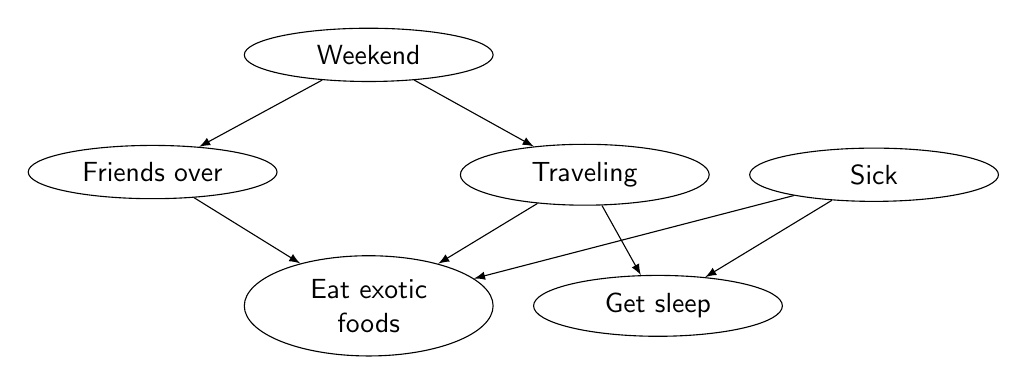
\begin{tikzpicture}[
    node distance=1cm and .5cm,
    bn/.style={draw,ellipse,text width=2cm,align=center}
      ]
      \node[bn] (w) {\attr{Weekend}};
      \node[bn,below right=of w] (t) {\attr{Traveling}};
      \node[bn,right=of t] (s) {\attr{Sick}};
      \node[bn,below left=of w] (f) {\attr{Friends over}};
      \node[bn,below right=of f] (eef) {\attr{Eat exotic foods}};
      \node[bn,right=of eef] (gs) {\attr{Get sleep}};
      \path (w) edge[-latex] (t)
      (w) edge[-latex] (f)
      (f) edge[-latex] (eef)
      (t) edge[-latex] (eef)
      (t) edge[-latex] (gs)
      (s) edge[-latex] (gs)
      (s) edge[-latex] (eef);
      \end{tikzpicture}
  \end{center}

  The random variables are:

  \begin{itemize}
  \item \attr{Weekend}: Is it the weekend?
  \item \attr{Friends over}: Does the person have friends over?
  \item \attr{Traveling}: Is the person traveling?
  \item \attr{Sick}: Is the person sick?
  \item \attr{Eat exotic foods}: Is the person eating exotic foods?
  \item \attr{Get Sleep}: Is the person getting sleep?
  \end{itemize}

  \medskip

  For the following questions, $A \perp B$ means that events A and B are
  independent and $A \perp B | C$ means that events A and B are independent
  conditioned on C.

  \textbf{Use the concept of d-separation} to answer the
  questions and show your work (i.e., state what the blocking path(s) is/are and what nodes block the path; or explain why each path is not blocked).

  \textit{Example Question:} Is $\attr{Friends over} \perp \attr{Traveling}$? If NO, give intuition for why.

  \textit{Example Answer:} NO. The path from Friends over -- Weekend -- Traveling is not blocked following the d-separation rules as we do not observe Weekend. Thus, the two are not independent. 

  \textbf{Actual Questions:}

\begin{enumerate}
\item Is $\attr{Weekend} \perp \attr{Get Sleep}$?
  If NO, give intuition for why.

\item Is $\attr{Sick} \perp \attr{Weekend}$?
  If NO, give intuition for why.


\item Is $\attr{Sick} \perp \attr{Friends over}\given \attr{Eat exotic
  foods}$? If NO, give intuition for why.


\item Is $\attr{Friends over} \perp \attr{Get Sleep}$? If NO, give
  intuition for why.

\item Is $\attr{Friends over} \perp \attr{Get Sleep} \given
  \attr{Traveling}$? If NO, give intuition for why.

\item Suppose the person stops traveling in ways that affect their
  sleep patterns.  Travel still
  affects whether they eat exotic foods.  Draw the modified network. (Feel free to reference the handout file for the commands for displaying the new network in \LaTeX).

\item For this modified network, is $\attr{Friends over} \perp
  \attr{Get Sleep}$? If NO, give an intuition why.  If YES,
  describe what observations (if any) would cause them to no longer be
  independent.

\end{enumerate}
\end{problem}

\subsection*{Solution}

\begin{enumerate}
  \item NO, they are not independent. The nodes \( \text{Weekend} \) and \( \text{Get Sleep} \) are connected through an intermediary node, say \( \text{Travel} \). Unless \( \text{Travel} \) is observed, it cannot be asserted independence between \( \text{Weekend} \) and \( \text{Get Sleep} \) due to the potential influence of \( \text{Travel} \) on both.
  \item YES. There is independence between \( I \) and \( H \) since they are connected through other nodes, such as "Weekend" (\( T \)) and "Sick" (\( R \)), which are not observed. Due to the lack of observation of these intermediate nodes, the path between \( I \) and \( H \) can't be deemed active, thus \( I \perp H \).
  \item NO. Observing "Eating Exotic Foods" (\( D \)) creates a dependency between two variables, say "Health" (\( H \)) and "Company" (\( C \)), since it acts as a collider, thereby allowing the flow of information between \( H \) and \( C \).
  \item NO. The independence between \( Friends \) and \( Get Sleep \) does not hold because the path through \( Weekend \) and \( Traveling \) is unblocked, implying a dependency due to the absence of observed intermediate nodes.
  \item YES. The observation of the node "Traveling" and "Weekend and "Get Sleep" being independent ensures conditional independence between \( having friends \) and \( weekend \) following d-separation rules.
  \item
  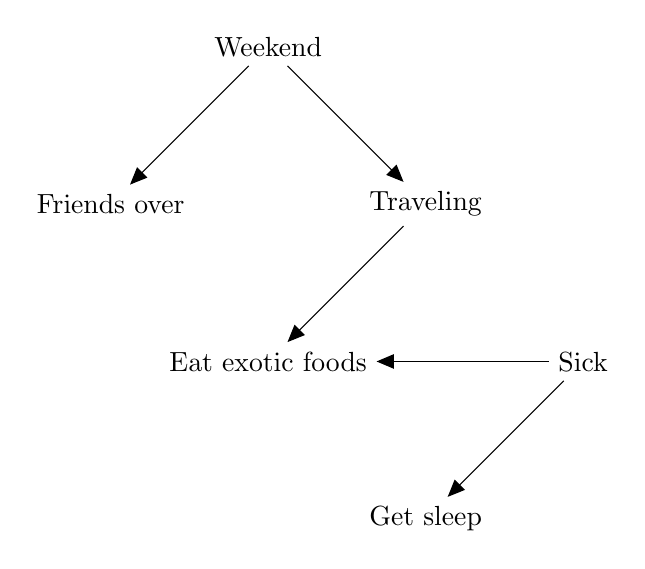
\begin{tikzpicture}
  %  Define nodes
  \node (weekend) at (0,0) {Weekend};
  \node (friendsover) at (-2,-2) {Friends over};
  \node (traveling) at (2,-2) {Traveling};
  \node (sick) at (4,-4) {Sick};
  \node (eatexoticfoods) at (0,-4) {Eat exotic foods};
  \node (getsleep) at (2,-6) {Get sleep};

  % Connect the nodes
  \draw[->] (weekend) -- (friendsover);
  \draw[->] (weekend) -- (traveling);
  \draw[->] (traveling) -- (eatexoticfoods);
  \draw[->] (sick) -- (eatexoticfoods); 
  \draw[->] (sick) -- (getsleep); 

  % Plates

\end{tikzpicture}
  \item Yes. Exotic foods is not observed, which means having friends over and the weekend are independent. Being sick would be dependent with having friends over if exotic foods had been observed. Sleep is a descendant of being sick, so it's independent of havng friends over. 
\end{enumerate}

\newpage


%%%%%%%%%%%%%%%%%%%%%%%%%%%%%%%%%%%%%%%%%%%%%
% Name and Calibration
%%%%%%%%%%%%%%%%%%%%%%%%%%%%%%%%%%%%%%%%%%%%%
\subsection*{Name} Shreshth Rajan 

\subsection*{Collaborators and Resources}
Whom did you work with, and did you use any resources beyond cs181-textbook and your notes? OH, Peter Pich 

\end{document}
